\chapter{Performance evaluation}

\section{Evaluation metrics}

The system is evaluated by checking how many landmarks are explored as time passes. A simulation is concluded when time reaches a maximum allowed value (3000). For example, if we have the following values:

\begin{center}
[100, 400, 800, 3000]
\end{center}

\noindent
The first landmark has been explored at time 100, etc. The last one has not been explored during the simulation, and so its value is set to 3000. This way, we can model the trend of the system using a time series where each time t is associated to the number of landmarks that had already been explored in such time. 

\noindent
Figure \ref{fig:ts} reports a clarifier example of a time series.

\begin{figure}[H]
\centering
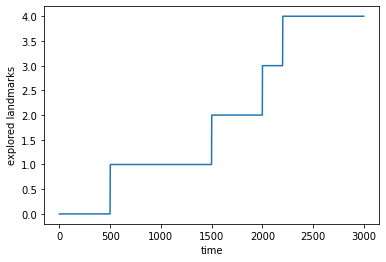
\includegraphics[width=8cm, keepaspectratio]{images/ts.png}
\caption{\textit{Example time series with exploration times [500, 1500, 2000, 2300].}}
\label{fig:ts}
\end{figure}

\smallskip
Moreover, we define a measure of performance (\textit{goodness}) to estimate how well the system behaves so that we can compare different combinations of parameters in a quantitative way. To do this, we consider the area under the time series (i.e., the integral of the function). Such area can assume values in range [0; 12000] (0 if no landmark has been explored during the simulation, 12000 is a theoretical max value given by $simulation\_length * n\_landmarks$). The main idea is that the greater the area, the sooner landmarks had been explored. Notice that, each value is then normalized in [0;1] for convenience.

\noindent 
Figure \ref{fig:auc} reports a clarifier example of lower and upper bounds.  

\begin{figure}[H]
\centering
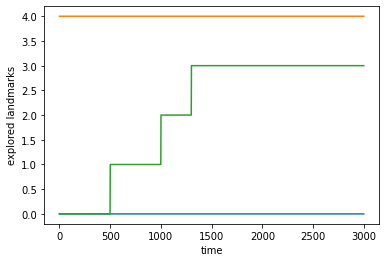
\includegraphics[width=8cm, keepaspectratio]{images/auc.png}
\caption{\textit{Example time series with exploration times [500, 1000, 1300, 3000] (green). Upper and bound bounds in orange and blue respectively. The integral of the blue function is simply 0, while the one of the orange is given by 3000 * 4.}}
\label{fig:auc}
\end{figure}

\noindent
\textit{Note:} Notice that, in order to compare solutions with different expected cluster size, such measure should be refined  since the latter parameter influences the exploration times in a non negligible manner. To overcome such issue, a penalty factor may be added to cluster with lower sizes. 

\section{Parameters definition}

When executing performance evaluation stage, we choose just a subset of parameters and configurations the system can be tuned upon since the total number of combination is exponential, and so it would require too much time to explore them all using a grid search technique. In particular, the following aspects are the one considered as constants:

\begin{itemize}

  \item Size of the arena: it is assumed to use a 4x4 meters arena.
  \item Position of the base: it is assumed to locate the base in the center of the arena.
  \item Few controller parameters: all non-deterministic transition parameters, gain factor in motor schema modules etc.
  \item Type of exploration: it may be interesting to test the system using different exploration strategies aside from the ballistic motion.
  \item Number of landmarks: it is assumed to have four landmarks  

\end{itemize} 

\noindent
The system is evaluated by changing the following parameters:

\begin{itemize}

  \item Number of employed robots: 20, 30, 40.
  \item Expected cluster size: 1, 3, 5.
  \item Number of obstacles scattered around the arena: 0, 10, 20
  \item Position of the landmarks 

\end{itemize}  

The first analyzed setup of the arena is reported in figure \ref{fig:arena}. The four landmarks are all placed on a same side of the arena and they are aligned so that a straight line parallel to one edge of the arena is created. Then, aside from this basic arena configuration, further evaluations will be made using different deployments of the landmarks (at the four cardinal points, at the four corners, random distribution etc.).  

\begin{figure}[H]
\centering

\includegraphics[width=\linewidth]{images/arena.png}
\caption{\textit{Setup of the arena with the four landmarks located on a straight line parallel to one edge of the arena.}}
\label{fig:arena}
\end{figure}

\section{Basic arena}

When considering the basic setup of the arena, table \ref{tab:perf-table} reports the \textit{minimum guaranteed level of service} (i.e. worst values among all the executed runs) and the goodness of each casuistry. Figure \ref{fig:ts-all} shows the comparison of the cases reported in table \ref{tab:perf-table}.

\bigskip
\noindent
\textbf{Number of robots}

An increase in the number of robots improves the overall performance values in general. 
Indeed, we can notice that the system can not reach the goal using cluster size three just when using twenty robots. Moreover, we obtain the best results when using the maximum number of robots (forty).
However, when dealing with an higher number of robots than forty and if keeping the same size of the arena, they may disturb each other, and so further evaluations should be made and no general rule can be inferred. 

Besides, notice that the minimum guaranteed level of service can be tricky. Indeed, by looking to raw performance data (available in attached files), it is confirmed that better average performance values are obtained despite a same minimum guaranteed level of service for cluster size five.

\bigskip
\noindent
\textbf{Cluster size}

As expected, exploration times increase proportionally to the cluster size. Indeed, aside from the trivial fact that more robots should gather, it is seen that the gathering operation itself is harder because of spatial constraints (harder for a robots to get close to a landmark if few robots are already there).

\noindent
An expected size greater than three makes the creation of a cluster harder, and often few landmarks remain unexplored at the ending of the simulation. As observed from empirical tests, such issue is mainly due to spatial problems constraints (difficulty to actually aggregate since there is not enough space). A greater time limit has been probed, and it emerged to be that clusters will be created anyway eventually. Moreover, few tests have been executed on wider arenas (e.g. 6x6, 8x8 meters) and, despite higher times due to the greater distances to travel, cluster creation resulted to be simplified.

\bigskip
\noindent
\textbf{Number of obstacles}

The insertion of obstacles is a key factor since it emerges a great difference among the study cases. Indeed, the performance will decrease independently from the adopted cluster size, and this is quite obvious since the boxes make exploration and aggregation harder (in some observed cases even impossible by leaving not enough empty space to create a proper cluster). However, notice that the gap between thirty and forty robots is filled up when using cluster size three or greater (rather, slightly better performance using thirty robots, 40 robots + 20 obstacle + 4 landmarks may create too harsh conditions for the navigation).

\bigskip
\noindent
\textbf{Miscellaneous}

\begin{itemize}

  \item As expected, the landmarks on the sides are often the last to be explored because their harder to reach (and it is harder to create cluster around them too).

\end{itemize}

\begin{table}[H]
\centering
\begin{tabular}{| c c c | c c c c | c |}

\hline
Robots & Cluster size & Obstacles & \multicolumn{4}{ c |}{Time} & Goodness \\
\hline
20 & 1 & 0  & 161& 258& 343& 1081 & 0.84 \\
20 & 1 & 10 & 300& 329& 1705& 1931& 0.64\\
20 & 1 & 20 & 266& 370& 863& 2771& 0.64\\
20 & 3 & 0  & 559& 1231& 2730& 3000& 0.37\\
20 & 3 & 10 & 3000& 3000& 3000& 3000& 0.0\\
20 & 3 & 20 & 3000& 3000& 3000& 3000& 0.0\\
20 & 5 & 0  & 3000& 3000& 3000& 3000& 0.0\\
20 & 5 & 10 & 3000& 3000& 3000& 3000& 0.0\\
20 & 5 & 20 & 3000& 3000& 3000& 3000& 0.0\\
\hline
30 & 1 & 0  & 115& 372& 414& 1032& 0.83\\
30 & 1 & 10 & 234& 418& 548& 2112& 0.72\\
30 & 1 & 20 & 317& 623& 994& 3000& 0.58\\
30 & 3 & 0  & 869& 1165& 2401& 3000& 0.33\\
30 & 3 & 10 & 1449& 1962& 2981& 3000& 0.21\\
30 & 3 & 20 & 1461& 2667& 2990& 3000& 0.15\\
30 & 5 & 0  & 3000& 3000& 3000& 3000& 0.0\\
30 & 5 & 10 & 3000& 3000& 3000& 3000& 0.0\\
30 & 5 & 20 & 3000& 3000& 3000& 3000& 0.0\\
\hline
40 & 1 & 0  & 175& 236& 367& 862& 0.86\\
40 & 1 & 10 & 268& 410& 420& 1022& 0.82\\
40 & 1 & 20 & 307& 580& 1018& 2069& 0.66\\
40 & 3 & 0  & 833& 834& 970& 2566& 0.53\\
40 & 3 & 10 & 1542& 1633& 2394& 2453& 0.33\\
40 & 3 & 20 & 1534& 2815& 3000& 3000& 0.13\\
40 & 5 & 0  & 3000& 3000& 3000& 3000& 0.0\\
40 & 5 & 10 & 3000& 3000& 3000& 3000& 0.0\\
40 & 5 & 20 & 3000& 3000& 3000& 3000& 0.0\\
\hline

\end{tabular}
\caption{\label{tab:perf-table}\textit{Evaluation of the system on 27 proposed combinations. For each casuistry, it is reported the moment of exploration of each landmark. Every value is the worst value among the registered ones. Moreover, the goodness of each combination is reported too.}}
\end{table}

\begin{figure}[H]
\centering
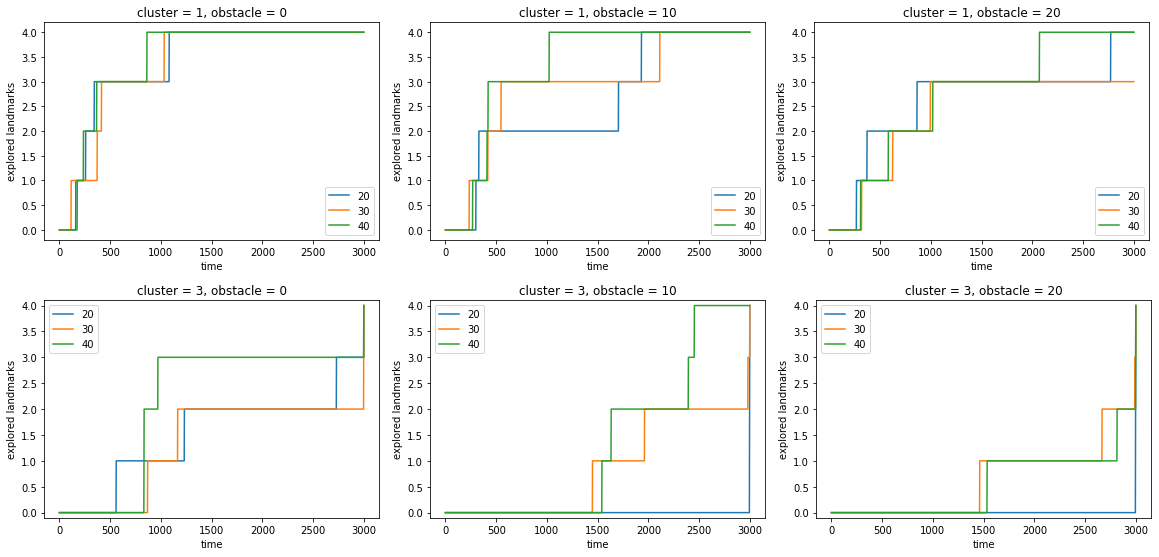
\includegraphics[width=\linewidth]{images/ts_all.png}
\caption{\textit{Performance on each casuistry using cluster size one and three for minimum guaranteed level of service (cluster size five is omitted since its values would always have been zero.}}
\label{fig:ts-all}
\end{figure}

\section{Further case studies}

Now, the system is probed using a different positioning of the landmarks in order to check its robustness on different cases. In particular, while fixing the cluster size to three and the number of obstacle to ten, the system is evaluated by choosing random locations for the landmarks. Configurations are dropped when the landmarks are spawned in the base or at least two of them are too close (because of possible interferences when counting neighbors through the range and bearing system). 

\noindent
Table \ref{tab:perf-table-random} reports the observed results. As we can notice, the positioning of the landmarks is a key factor since it greatly influences the results. Indeed, the goodness assumes very high/low values depending on very lick/unlucky configurations, and so the variance between the exploration times is higher than the one observed when just using the basic arena. 

\noindent
Moreover, as expected, the system behaves better when employing the maximum number of robots (forty). 

\bigskip
When comparing such results to the ones obtained on the basic arena (figure \ref{fig:ts-random}), it emerges that better results are generally obtained on the random ones: this is probably due to the fact that, since in the basic arena all landmarks are placed on the same side, robots that start exploring the opposite part will not find any landmark for a while, and so they are vain for the first part of the simulation. Obviously, such considerations can not be made for random deployment of the landmarks in general, and so better performance are obtained since all robots take part in the creation of the clusters. In the end, notice that the clustering behavior emerges independently from the number of robots when using random arenas, while it is not true when using twenty robots on the basic arena (at least in the specified time boundaries).

\bigskip
\noindent
\textit{Note:} Such evaluations may be tricky (or even misleading) since more attempts on further cases should be made in order to apply any statical technique to validate the results.

\begin{table}[H]
\centering
\begin{tabular}{| c c c | c c c c | c |}

\hline
Robots & Cluster size & Obstacles & \multicolumn{4}{ c |}{Time} & Goodness \\
\hline

\multirow{5}{4em}{20} & \multirow{5}{4em}{3} & \multirow{5}{4em}{10} & 231& 886& 2388& 3000& 0.45\\
& & & 396& 640& 3000& 3000 & 0.41\\
& & & 112& 975& 2645& 2871 & 0.45\\
& & & 454& 1112& 1921& 2678 & 0.48\\
& & & 432& 1001& 2319& 2992 & 0.43\\
\hline

\multirow{5}{4em}{30} & \multirow{5}{4em}{3} & \multirow{5}{4em}{10} & 325& 344& 1481& 1684& 0.68\\
& & & 101& 863& 907& 3000& 0.59\\
& & & 494& 653& 3000& 3000& 0.40\\
& & & 575& 1166& 3000& 3000& 0.35\\
& & & 1310& 1667& 1718& 3000& 0.40\\
\hline

\multirow{5}{4em}{40} & \multirow{5}{4em}{3} & \multirow{5}{4em}{10} & 524& 800& 815& 1060& 0.73\\
& & & 183& 942& 2445& 2771& 0.47\\
& & & 529& 854& 1926& 2714& 0.49\\
& & & 960& 1278& 2167& 3000& 0.38\\
& & & 102& 672& 719& 3000& 0.62\\
\hline

\end{tabular}
\caption{\label{tab:perf-table-random}\textit{Evaluation of the system using random positioning of the landmarks. For each casuistry, it is reported the moment of exploration of each landmark for a random setup of the landamrks. Moreover, the goodness of each combination is reported too.}}
\end{table} 

\begin{figure}[H]
\centering
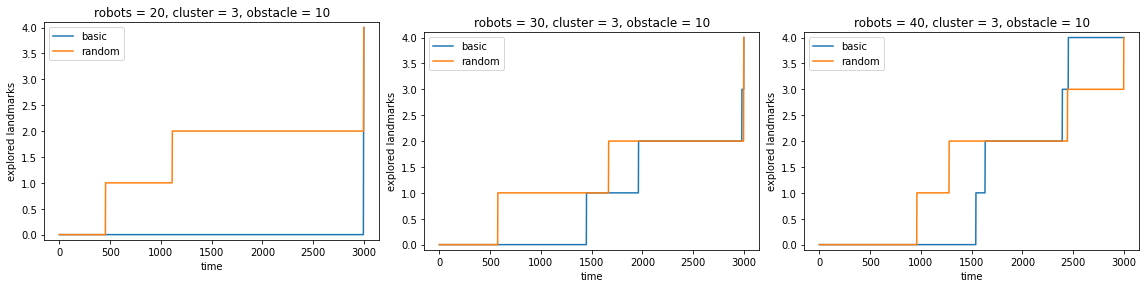
\includegraphics[width=\linewidth]{images/ts_random.png}
\caption{\textit{Comparison of the performance obtained on basic arena and on random ones.}}
\label{fig:ts-random}
\end{figure}


